% Clean CV/Resume Template, by Bennet B <dev@bennet.cc>
% CC0, Public-Domain
% 
% Permission is hereby granted, free of charge, to any person obtaining a copy
% of this template and associated files (the "Template"), to deal
% in the Template without restriction, including without limitation the rights
% to use, copy, modify, merge, publish, distribute, sublicense, and/or sell
% copies of the Template, and to permit persons to whom the Template is
% furnished to do so, subject to the following conditions:
%
% The above copyright notice and this permission notice shall be included in all
% copies or substantial portions of the Template.
%
% THE TEMPLATE IS PROVIDED "AS IS", WITHOUT WARRANTY OF ANY KIND, EXPRESS OR
% IMPLIED, INCLUDING BUT NOT LIMITED TO THE WARRANTIES OF MERCHANTABILITY,
% FITNESS FOR A PARTICULAR PURPOSE AND NONINFRINGEMENT. IN NO EVENT SHALL THE
% AUTHORS OR COPYRIGHT HOLDERS BE LIABLE FOR ANY CLAIM, DAMAGES OR OTHER
% LIABILITY, WHETHER IN AN ACTION OF CONTRACT, TORT OR OTHERWISE, ARISING FROM,
% OUT OF OR IN CONNECTION WITH THE TEMPLATE OR THE USE OR OTHER DEALINGS IN THE
% TEMPLATE.
%
% based on Modern CV by Habib Semouma
% https://www.overleaf.com/latex/templates/modern-cv-slash-resume-template/vjrqdkpjckwj
%
% 
\documentclass[oneside]{article}

\usepackage{fontspec}
\usepackage{wallpaper}
\usepackage{geometry}
\usepackage[
    unicode=true,
    bookmarks=true,
    bookmarksnumbered=false,
    bookmarksopen=true,
    bookmarksopenlevel=1,
    breaklinks=false,
    pdfborder={0 0 0},
    backref=false,
    colorlinks=false
    ]{hyperref}
\usepackage{lastpage}
\usepackage{hyphenat}
\usepackage{hyphsubst}
\usepackage{tabularx}
\usepackage{moresize}
\usepackage[document]{ragged2e}
% \usepackage{parskip}

\usepackage[scaled]{helvet}
\usepackage{fontawesome5}
\usepackage{academicons}
\usepackage[defaultfam,tabular,oldstyle]{montserrat}
\usepackage[T1]{fontenc}
\renewcommand*\oldstylenums[1]{{\fontfamily{Montserrat-TOsF}\selectfont #1}}

\usepackage{titlesec}
\usepackage{xcolor}
\usepackage{tikz}

\setlength{\parindent}{0pt}
\titleformat{\section}{\normalfont}{}{0pt}{}

\renewcommand{\arraystretch}{1.4}

\setlength\fboxrule{0pt}
\setlength\fboxsep{12pt}
% \setlength{\parskip}{.5\baselineskip plus 2pt}
% \renewcommand{\baselinestretch}{1.1}

\titlespacing{\section}{0pt}{1.5ex plus .1ex minus .2ex}{1pc}

\newcolumntype{Y}{>{\RaggedRight\arraybackslash}X}

% Change PDF Meta Info here
\hypersetup{
    pdftitle={Mario Grandi - CV - English},
    pdfauthor={Mario Grandi},
    pdfsubject={CV}
}

% Paper size
\geometry{
    a4paper,
    left=0pt,
    right=0pt,
    top=0pt,
    bottom=0pt,
    nohead,
    % includefoot,
    nomarginpar
}

% Background Color of the Sidebar Column
\definecolor{sidebg}{cmyk}{1, 0.02, 0, 0.56}
% Background Color of the Main Column
\definecolor{mainbg}{cmyk}{0, 0, 0.07, 0.04}

% Text Color of the Main Column
\definecolor{maintext}{cmyk}{1, 0.02, 0, 0.8}
% Text Color of the Sidebar Column
\definecolor{sidetext}{cmyk}{0, 0, 0.07, 0.04}

\pagecolor{mainbg}

% Build custom made command for quick employment history inputs
\newcommand{\empitem}[7]{
        {\large \textbf{#1,}} 
        {{\fontseries{light}\selectfont #2}}\\
        {{\fontseries{medium}\selectfont #3}} \\
        {\scshape\fontseries{light}\selectfont\footnotesize #4 \textendash{} #5 (#6)} 
        #7
}

\begin{document}
\setlength{\topskip}{0pt}\setlength{\footskip}{0pt}%
\fcolorbox{red}{sidebg}{%
    \begin{minipage}[t][\textheight-2\fboxsep-2\fboxrule][t]{\dimexpr0.40\textwidth-2\fboxrule-2\fboxsep\relax}
        \color{sidetext}
        %%%%%%%%%%%%%%%%%%%%%%%%%%%%%%%%%%%%%%%%%%%%%%%%%%%%
        % YOUR NAME, PRONOUNS, OCCUPATION(s), AND HEADSHOT
        {\bfseries\scshape\HUGE Mario} \\
        {\bfseries\scshape\Huge Grandi}
        \vspace{.3cm} \\
        \begin{center}
            \begin{tikzpicture}
            \clip (0,0) circle (3.5cm) node[anchor=center] {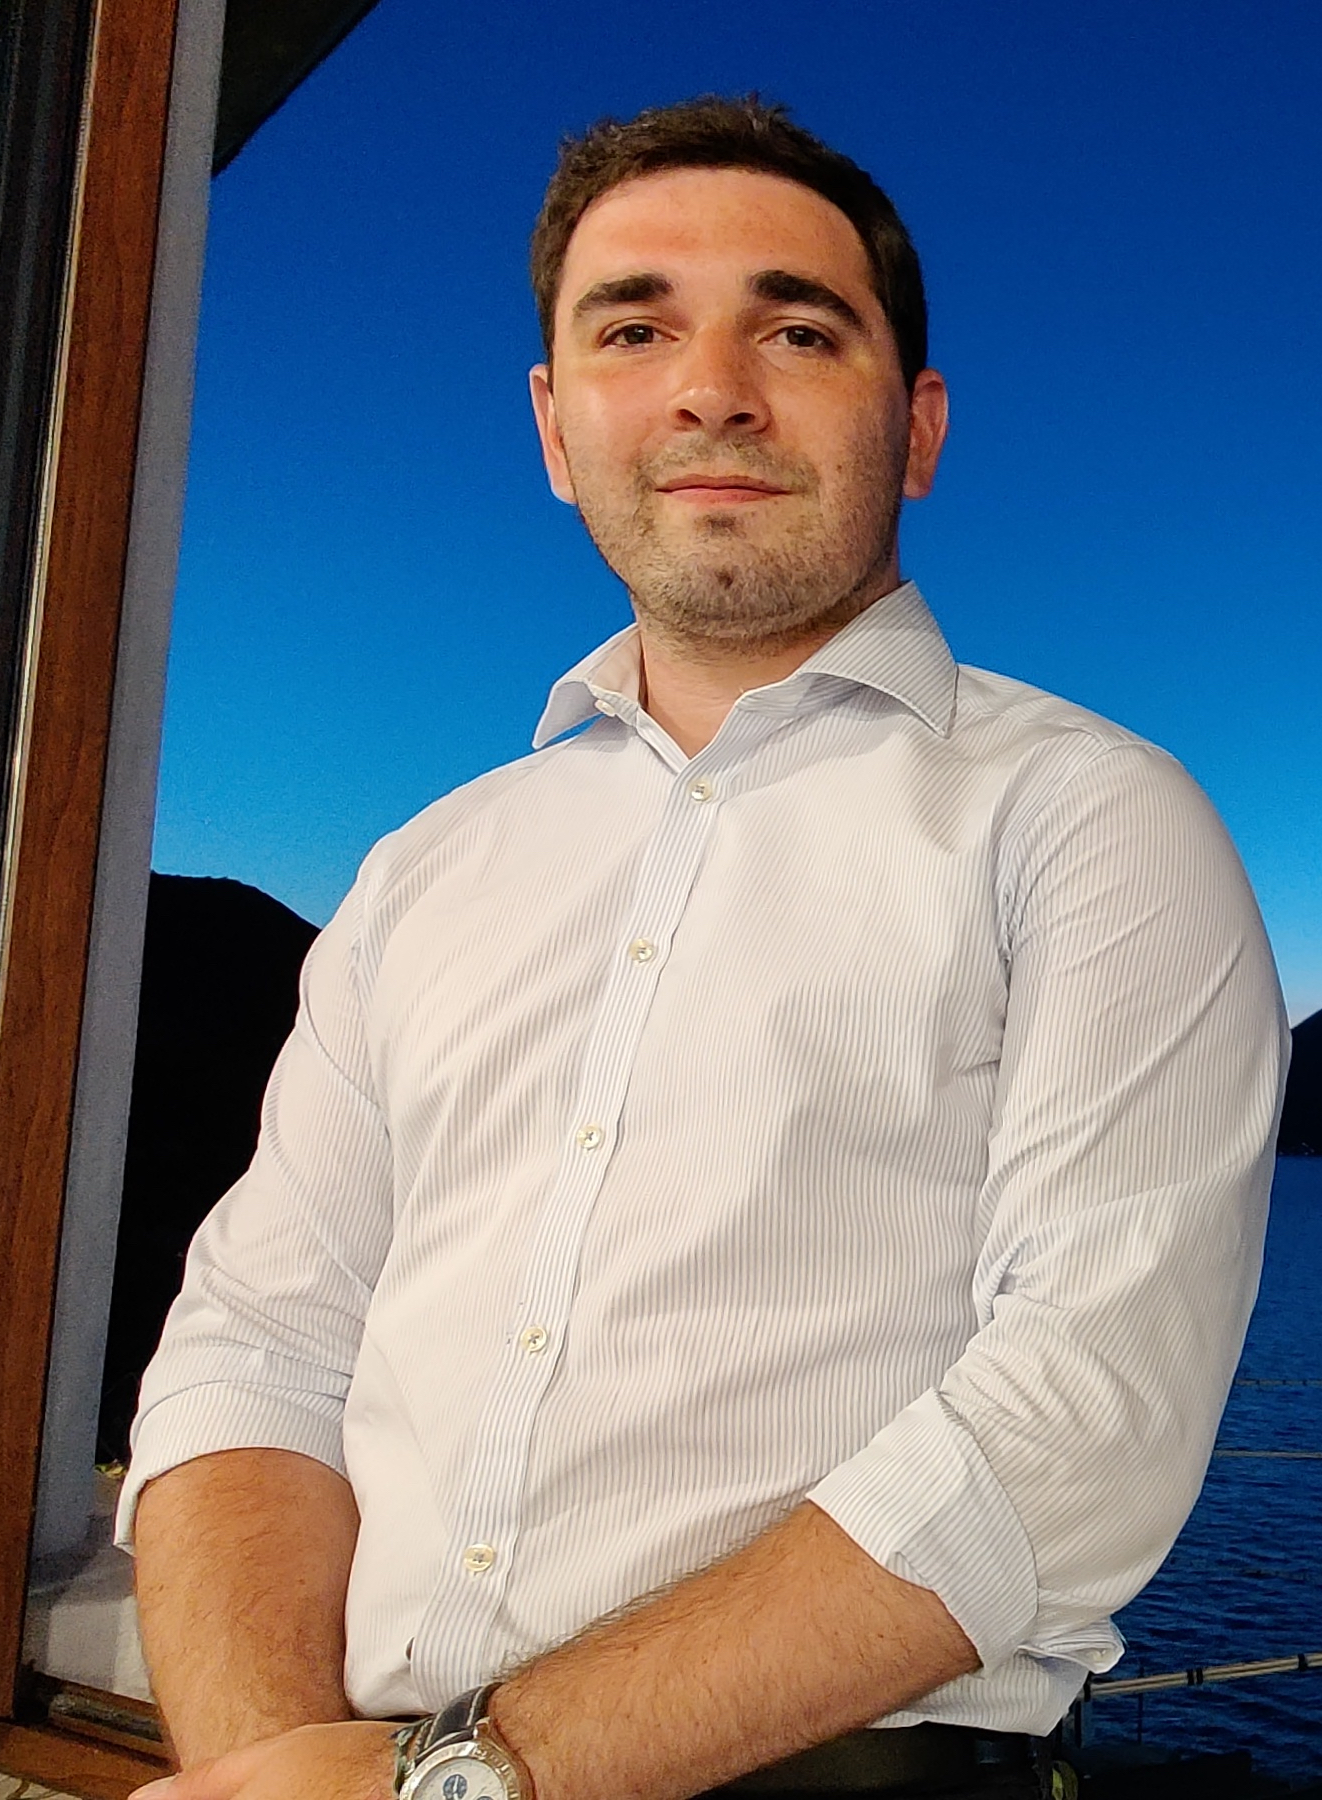
\includegraphics[trim=0cm 15cm 0cm 0cm, clip=True, width=7cm]{mario_grandi.jpeg}}; 
            \end{tikzpicture}
        \end{center}
        \vspace{.3cm}
        %%%%%%%%%%%%%%%%%%%%%%%%%%%%%%%%%%%%%%%%%%%%%%%%%%%%
        % YOUR PERSONAL INFROMATION
        \phantomsection{}
        \addcontentsline{toc}{section}{Personal info}
        \section*{\large Personal info}
        \begin{tabularx}{\textwidth}{cY}
            \faicon{Phone}      & +44 (0)7999206347 \\
            \faicon{envelope}   & \href{mailto:dr.mario.grandi@gmail.com}{dr.mario.grandi@gmail.com} \\
            \faicon{mapmarker}  & 45a Borough Street, Brighton\\
            & BN1 3BG, United Kingdom \\
        \end{tabularx}
        \vspace{.3cm} \\
        \rule{\linewidth}{0.4pt} \\
        %%%%%%%%%%%%%%%%%%%%%%%%%%%%%%%%%%%%%%%%%%%%%%%%%%%%%%%%%
        % YOUR LINKS, YOU MAY ALSO ADD A PERSONAL WEBSITE OR PORTFOLIO
        \phantomsection{}
        \addcontentsline{toc}{section}{Links}
        \section*{\large Links}
        \begin{tabular}{cl}
        %    \faCode{}     & \href{https://example.com}{example.com}
            \faicon{github}   & \href{https://github.com/mg380}{https://github.com/mg380} \\
            \faicon{linkedin} & \href{https://www.linkedin.com/in/mario-grandi/}{www.linkedin.com/in/mario-grandi} \\
            \aiOrcid{}     & \href{https://orcid.org/0000-0002-5924-2544}{0000-0002-5924-2544} \\
        \end{tabular}
        \vspace{10pt} \\
        \rule{\linewidth}{0.4pt} \\
        %%%%%%%%%%%%%%%%%%%%%%%%%%%%%%%%%%%%%%%%%%%%%%%%%%%%%%%%%%%%
        % YOUR SKILLS
        % Add/Remove as seen fit, Icons: https://packages.oth-regensburg.de/ctan/fonts/fontawesome5/doc/fontawesome5.pdf
        \phantomsection{}
        \addcontentsline{toc}{section}{Skills}
        \section*{\large Skills}
        \begin{tabularx}{\textwidth}{cY}
            \faicon{code}        & Python - C++ - Bash - MySQL - SQL - AWS - Git/GitHub/GitLab - Microsoft Excel \\
            \faicon{toolbox}     & TensorFlow - Keras - Pandas - Scipy - Numpy - OpenCL - pyOpenCL - OpenMP - Vitis HLS \\ 
            \faicon{cogs}        & Machine Learning - Statistics - Monte Carlo Simulations - Distributed Computing - Data Science Methods - Big-Data Analysis - Data Visualisation - Communication - Teamwork \\
            \faicon{pen}        & \LaTeX - Microsoft Studio Office - Keynote\\
            \faicon{LaptopCode}  & Linux - Windows - macOS \\
        \end{tabularx}
        \vspace{1pt} \\
        \rule{\linewidth}{0.4pt}
        %%%%%%%%%%%%%%%%%%%%%%%%%%%%%%%%%%%%%%%%%%%%%%%%%%%%%%%%%%%%%%%%
        % GRADESCALE (if nesseary, e.g. if you apply abroad, where scales 
        % are different. You should at least provide, what the best possible
        % grade and what the worst possible grade is)
    \end{minipage}
}
\hfill
\fcolorbox{red}{mainbg}{%
    \begin{minipage}[t][\dimexpr\textheight-2\fboxrule-2\fboxsep\relax][t]{\dimexpr0.6\textwidth-2\fboxrule-2\fboxsep\relax}
        \color{maintext}
        %%%%%%%%%%%%%%%%%%%%%%%%%%%%%%%%%%%%%%%%%%%%%%%%%%%%%%%%%%
        % WORK EXPERIENCE
        \phantomsection{}
        \addcontentsline{toc}{section}{Employment History}
        \section*{\scshape\Large Employment History \rule{\linewidth}{0.4pt}}
%
        \empitem{QA-UK Ltd}
        {London, United Kingdom}
        {Head of Analytics}
        {May 2023}
        {ongoing}
        {Fulltime}
        {
        \begin{itemize}
            \setlength{\itemsep}{-3pt}
            \item Working as the lead researcher for the company in driving all project pipelines from planning to deliverables, investigating and prototyping new technologies, and analysing collected data for the full stack of green technologies portfolio.
            \item Implemented and analysed complex fluid, thermal, and optical simulation using parallelisation techniques on AWS and large High-Performance Computing systems. 
            \item Aided in the negotiation and implementation of software license extension, delivering 25\% additional simulation time at no extra cost.   
            \item Led the testing and analysis of a prototype for a multi-million dollar green energy project and presented results to investors and stakeholders.
        \end{itemize}
        }
%
        \empitem{Office for National Statistics}
        {Titchfield, United Kingdom}
        {Statistical Production Analyst}
        {Sept 2022}
        {Mar 2023}
        {Fulltime Contractor}
        {
        \begin{itemize}
            \setlength{\itemsep}{-3pt}
            \item Was the co-lead of an 8-member team in charge of the collection and analysis of international trade data and provide effective insight, used by over 5 external clients and 2 internal branches to make government-wide decisions.
            \item Improved code quality through automated testing, reviewing, and validation.
            \item Produced clean and error-free Python code using Git for version control, to streamline data analysis and improve internal quality coding standards.
            \item Collaborated with 3 cross-platform professionals in an Agile environment and with a strict schedule, to oversee the successful delivery of requirements needed for a new software analysis platform.
            \item Identified several areas of improvement in the used statistical analysis methods and implemented cost-effective solutions.
            \item Streamlined pipeline processes using the Pandas Python library to reduce overall production and preparation time by over two weeks.
        \end{itemize}
        }
%
        \empitem{University of Sussex}
        {Brighton, United Kingdom}
        {Post-Doctoral Research Fellow}
        {Aug 2021}
        {Aug 2022}
        {Fulltime}
        {
        \begin{itemize}
            \setlength{\itemsep}{-3pt}
            \item Created a complex tracking algorithm in Python and C++, accelerated on FPGA hardware using HLS and on software using OpenCL and OpenMP.
            \item Achieved a decrease in the processing latency by a factor of 15 compared to software and occupy less than 50\% of available hardware resources.
            \item Maintained Linux-based server system hosting accelerator cards interfaced with a distributed computing system to streamline computation.
            \item Developed large-scale statically accurate Monte Carlo physics simulations using C++ and Python to test the performance of the developed algorithms.
            \item Successfully delivered the final product and presented final results to the funding agents and collaboration stakeholders, ensuring the programme's continued funding.
            \item Provided support and training for master and final year physics students.
        \end{itemize}
        }
        \vfill%
        {\hfill\small\fontseries{extralight}\selectfont Page \thepage of \pageref{LastPage}\hfill}
    \end{minipage}
}

\newpage

%%%%%%%%%%%%%%%%%%%%%%%%%%%%%%%%%
% PAGE 2
%%%%%%%%%%%%%%%%%%%%%%%%%%%%%%%%%
\fcolorbox{red}{mainbg}{%
    \begin{minipage}[t][\dimexpr\textheight-2\fboxrule-2\fboxsep\relax][t]{\dimexpr0.6\textwidth-2\fboxrule-2\fboxsep\relax}
        \color{maintext}
        % \vspace{.6cm}
        \empitem{Public Health England}
        {Cambridge, United Kingdom}
        {Data Scientist}
        {Jun 2019}
        {Sept 2019}
        {Internship}
        {
        \begin{itemize}
            \setlength{\itemsep}{-3pt}
            \item Developed and trained a Python-based Machine Learning algorithm using TensorFlow and Keras to simulate statistically significant and anonymised synthetic patient data from sensitive patient health data.
            \item Used data science analysis techniques in Python and Jupyter to define data integrity, data leakage and statistical resemblance and delivered the framework to the production team to enable them to draw meaningful conclusions and provide actionable recommendations to stakeholders and research partners.
            \item Monitored and optimise ML training and development using cometML
            \item Analysed and synthesised patient data with SQL tables, views, and Jupyter Notebooks in Python to provide insightful reports on its statical properties to team and stockholders.
            \item Documented full system analysis, testing, and implementation for production team handover.
        \end{itemize}
        }
        \empitem{University of Sussex}
        {Brighton, United Kingdom}
        {High Energy Physics PhD Researcher}
        {Sept 2017}
        {Jul 2021}
        {Fulltime}
        {
        \begin{itemize}
            \setlength{\itemsep}{-3pt}
            \item Performed large-scale data analysis using data science methods and skills on petabytes of data collected by the ATLAS experiment at CERN to perform feature extraction, data cleaning and transformation, and maximise experimental sensitivity.
            \item Used CI/CD with GitLab to help develop and implement C++, Python, and Bash C++ code to perform cut-based statistical analyses and machine learning based identification methods to discriminate events with very rare theoretically predicted particles from large background of standard model physics.
            \item Received extensive training in big data analysis, machine learning, and high- performance computing techniques through the DISCnet bursary programme.
            \item Maintained and improved on large analysis framework using coding best practices and large-scale project management with JIRA and GitLab to resolve bugs and issues quickly and effectively.
            \item Presented the work at several workshops, group meetings, and international conferences.
            \item The results of my analyses have been published in several respected physics journals.
        \end{itemize}
        }
    %%%%%%%%%%%%%%%%%%%%%%%%%%%%%%%%%%%%%%%%%%%%%%%%%%%%%%%%%%%
        % EDUCATION
        \phantomsection{}
        \addcontentsline{toc}{section}{Education}
        \section*{\scshape\Large Education \rule{.5\linewidth}{0.4pt}}
%
        {\large \textbf{PhD in Particle Physics, University of Sussex}} \\ {(Doctorate)}
        {\scshape\fontseries{light}\selectfont\footnotesize Sept 2017 \textendash{} Jul 2021} \\
        {\textit{Search for supersymmetry with the ATLAS detector at the Large Hadron Collider in final states with two hadronically decaying $\tau$-leptons.}} \\
        
        {\large \textbf{MPhys in Physics and Astrophysics, University of Sussex}} \\ {(Masters)}
        {\scshape\fontseries{light}\selectfont\footnotesize Sept 2013 \textendash{} Aug 2017} \\
        {\textit{Grade: 1$^{st}$ class degree with honours.}} \\

        {\large \textbf{International Baccalaureate, International School of Geneva}} \\ {(Ceritificate of Education)}
        {\scshape\fontseries{light}\selectfont\footnotesize Sept 2011 \textendash{} Aug 2013} \\
        {\footnotesize Higher Level subject: Physics, Mathematics, Economics} \\
        {\footnotesize Standard Level subjects: English, Spanish, Chemistry} \\
        {\textit{Grade: 34}} \\
        \vfill%
        {\hfill\small\fontseries{extralight}\selectfont Page \thepage of \pageref{LastPage}\hfill}
    \end{minipage}
}
\hfill%
\fcolorbox{red}{sidebg}{%
    \begin{minipage}[t][\dimexpr\textheight-2\fboxrule-2\fboxsep\relax][t]{\dimexpr0.4\textwidth-2\fboxrule-2\fboxsep\relax}
        \color{sidetext}
        % \vspace{.5cm}
        %%%%%%%%%%%%%%%%%%%%%%%%%%%%%%%%%%%%%%%%%%%%%%%%%%%%%%%%
        % YOUR NAME AND PREFERED PRONOUS AGAIN AS HEADER
        {\bfseries\scshape\HUGE Mario} \\
        {\bfseries\scshape\Huge Grandi}
        \vspace{.3cm} \\
        %%%%%%%%%%%%%%%%%%%%%%%%%%%%%%%%%%%%%%%%%%%%%%%%%%%%%%%%%%
        % LANGUAGES
        \phantomsection
        \addcontentsline{toc}{section}{Languages}
        \section*{\large Languages}
        \begin{tabular}{cl}
            \faicon{language} & English (Native) \\
            \faicon{language} & Italian (Native) \\
            \faicon{language} & French  (Advanced) \\
            \faicon{language} & Spanish (Intermediate) \\
        \end{tabular}
        \vspace{.3cm}
        \\
        \rule{\linewidth}{0.4pt}
        \\
        %%%%%%%%%%%%%%%%%%%%%%%%%%%%%%%%%%%%%%%%%%%%%%%%%%%%%%%%%%%%
        % CERTIFICATES AND AWARDS RECEIVED
        \phantomsection
        \addcontentsline{toc}{section}{Interest and Accomplishments}
        \section*{\large Interest and Accomplishments}
        \begin{tabularx}{\textwidth}{cY}
            \faicon{asterisk} & Analysed heath data collected by Terre Innovative Healthcare P.A.N.D.A. project to derive insight to better understand pregnancy related issues in rural countries and areas.\\
            \faicon{asterisk} & Developed, trained, and tested a CNN Machine Learning algorithm to automatically identify brain vesicles dyed with chemical compounds for Alzheimer's identification. \\
            \faicon{asterisk} & Winner of the Outreach Activity Project at the 2019 European School of High Energy Physics.\\
            \faicon{asterisk} & awarded the “All-round Middle Year Program Student" award.\\
            \faicon{asterisk} & Annual collaboration with “Progetti ECAR Mandabe” to organise fund-raising events for the village of Mandabe in Madagascar.\\
        \end{tabularx}
        \vspace{.3cm}
        \\
        \rule{\linewidth}{0.4pt}
    \end{minipage}%
}%
\end{document}